\documentclass{sig-alternate}
\def\allfiles{}
\usepackage{latexsym}
\usepackage{amsmath}
\usepackage{algorithm,algorithmic}
\usepackage{graphicx}
\usepackage{url}
\usepackage{subfigure}

\title{Extracting User's Hidden Profile on Twitter}

\author{
Dong Wang, Mohan Yang, Yuchen Liu
\and
\alignauthor
\affaddr{Department of Computer Science}\\
\affaddr{University of California, Los Angeles}\\
\email{\{dongw, yang, yliu\}@cs.ucla.edu}
}

\begin{document}

\maketitle

\begin{abstract}
In a social network environment like Twitter and Facebook, user modeling is an essential approach to know a user's interests, and thus making other additional services such as recommendation system possible and accurate. In user modeling, user profile is an important factor since it's written by user and it provides pretty accurate information. Previous social network websites such as Facebook and MySpace build a detailed profile when a user starts to use, letting a user fill in his/her personal information, education and work, family information as well as interests. However, Twitter has a different setting for user profile and it only allows a user to fill in a short bio within 160 characters to describe him/herself. Without the structured information, it's getting harder to build an accurate user profile. Meanwhile, according to our statistics, about 27.2\% of users do not have a self-written bio or their bio is less than 5 characters and about 43.9\% of users don't have a meaningful bio description since there are less than 10 characters in their bio. Thus, it becomes important for us to extract useful user profile for those who don't have a meaningful bio in order to model users accurately. In this paper, we propose approaches and models in two different categories, using social network link structure only and using user-generated content only, respectively. We also propose a co-training model to combine approaches in these two categories to make use of their advantages to achieve a better performance. In our UCLA dataset, co-training model performs a 87\% precison at top 50 results, which give out a promising results for extracting users' hidden profile problem.
\end{abstract}

\section{Introduction}

Twitter, a micro-blogging system combining social network and text content, has demonstrated itself as a leading breaking news provider, and a platform of sharing opinions and interests. Currently, according to Twitter Blog\cite{twitterblog}, there are about over millions of users publishing more than 200 millions of tweets on Twitter every single day. Although there are existing successful social networks websites before Twitter comes out, like Facebook, MySpace etc., Twitter becomes popular because of its simplicity and people find it easy to tweet and share information. There are several characteristics which differentiate Twitter with other social networks:

\begin{itemize}

\item \textbf{Non-Reciprocal Relationship: } In Twitter, users are connected with links called "follow". If user A is following user B, all tweets which are produced by B will appear in user A's timeline. However, this "follow" link does not require user B's permission and also B is not required to follow back. This characteristic means a user could follow anyone he/she is interested in freely. In Facebook or MySpace, users are connected by "friendship" and this link relationship is reciprocal meaning that two users need to agree with each other to be in such a "friendship".

\item \textbf{Incomplete Profile: } As Facebook provides a detailed profile covering personal information, family, education and work, interests, Twitter provides a simple bio information for user to describe him/herself. However, the bio information in Twitter is limited by 160 characters and does not contain any structured format. This short bio will make it difficult to know a user's profile, including affilication, occupation, interests etc., and thus hard for us to make more services, such as recommendation.

\item \textbf{User-generated Content as Plain Text: } While Facebook allows users to post different types of user-generated contents, such as status, photos, videos and external urls, Twitter only has one form of user-generated content - plain text data within 140 characters (so-called tweet). However, users could insert shortened urls of an image, a video or a webpage into tweets. This allows us to analyze users' tweets easily with only text data but also make it hard to target users' interests in a specific area, like music or movies.

\end{itemize}

User profiles act as an important factor in user modeling since the profile is completed by users and often is of good quality. With an accurate user modeling, many useful applications could be accomplished such as recommendation systems, advertisement delivery, information prioritization. However, as mentioned above, the design of short bio in Twitter makes it difficult to know a user's real information. According to our experiment, about 27.2\% of users don't have a self-written bio or their bio is less than 5 characters. About 43.9\% of users have a bio less than 10 characters, which indicates that almost half of users don't have a meaningful bio to describe themselves. In order to cope this problem, we could make use of the structure of the social network as well as the content information in users' tweets to extract such hidden profile for those who don't have a informative bio because they are lazy or they don't want to post those information. For example, if a user is studying at UCLA, even though he/she might not explicitly write this fact in his/her bio, we may find the following observations from his/her activities in Twitter:

\begin{enumerate}

\item In his/her social networks, including users he/she is following and users who is following him/her. there might be a considerate amount of users who is explicitly indicating they are students at UCLA.
\item In his/her tweets, she/he might post about what's happening in UCLA or something related to UCLA which could infer that she/he is a student at UCLA. She/he could also retweet tweets containing such information.

\end{enumerate}

Based on above observations, in this paper, we explore models and approaches to extract user's hidden profile from what they are connected in the social networks and what they are tweeting on Twitter. Specifically, on a social network graph, given a category and a set of seed users in the category, we want to find users in the graph who is likely to belong to this category and give out a ranking of users based on how likely they are to be in this category. In our solution, the approaches could be divided into two categories: 1) exploiting link structure in the graph only; 2) exploiting user-generated content information only, including bio, location and tweets. After describing three models in the above two categories, we also propose a co-training algorithm to combine the advantages of models in both categories to achieve a better performance with iterative reinforcing the result of one algorithm by the result of the other algorithms. With the help of information from both perspectives, we are achieving a 87\%  result at top-50 precison metric for UCLA dataset.

% User on Facebook has a complete profile by filling out his education, work and interest, while Twitter user can only fill out a piece of 160 characters bio information. It is difficult to precisely recommend related users, news and services on Twitter with limited user profile information. Thus, extracting a user's hidden profile is a valuable topic which improves user experience and advertisement revenue at the same time. Additionally, it will also help to improve the search result relevance by assigning a higher rank to the results in which the user is more interested.

% We will propose an algorithm to extract a user's hidden profile from his followers and followings using the closeness and tweets similarity of two users, which is based on the intuition that people with similar background and interests tend to connect with each other.

%However, proposing an efficient solution to the problem is very challenging due to sparseness and incompleteness of the following relation data. The Twitter network graph is a very large but spare graph which involves over a hundred million users, while most of them are connected to only hundreds of users. Additionally, some users have more than a thousand followers which cannot be completely retrieved due to the limit of Twitter API. Thus, our algorithm should be able to predict with sparse and incomplete following relation data.

The rest of the paper is organized as follows.
Section~\ref{sec:problem} presents the mathematical formulation of the problem. Section~\ref{sec:method} presents four solutions to this problem. Section~\ref{sec:experiment} reports the experiment results. Section~\ref{sec:discussion} discusses some problems discovered in the experiment. The paper concludes in Section~\ref{sec:conclusion}.

%Section \ref{sec:related-work} compares our work with related work.

\section{Problem Formulation}\label{sec:problem}

abc
\ifx \allfiles \undefined
\documentclass{article}
\usepackage{booktabs}
\usepackage{multirow}
\usepackage{graphicx}

\begin{document}
\title{Method}
\maketitle \else \fi

\section{Our Approach}\label{sec:method}

%I think we need rewrite this part. Thanks.

%Our crawler will begin with Twitter users from four universities including UCLA, USC, Stanford and MIT, and perform a two-step random walk starting from these users to obtain a larger set of different background users. Every user's profile, followers and followings information will be retrieved. The crawler will also retrieve these users' tweets posted after a specific time.
%We will analysis the number of followers, followings, tweets and retweets for each user, and quantify a user's influence on these metrics using a PageRank like mechanism.
%We will analysis the tweet keywords for each user, and provide a metric to evaluate the tweets similarity between two users. We will also compare the interest difference between users in different universities.
%We will quantify two users' closeness using their tweet and reply (regarding retweet as a kind of reply) behavior data. Our model is similar to the model used in predicting a chess game result based on two players' past campaign results \cite{elo1986rating}.
%We will propose an algorithm for extracting a user's hidden profile. Each edge will be weighted by the closeness and tweets similarity of the corresponding two users. The algorithm performs a random walk on the weighted graph to collect all possible hidden profile for a specific user.

\subsection{Data Collection}
We selected 20 seed users from each of the four universities, including UCLA, USC, Stanford and MIT. User profile (id, location, screen name, number of followings and followers, and a short biography) of these seed users was crawled using the Twitter API. Starting from these seed users, a two-step random walk is performed to retrieve their followers and their followers' followers. If a new user from these four universities is discovered during the procedure, this user is marked as a seed user and another two-step random walk starting from this user is performed. The crawler has collected more than 540,000 users and 780,000,000 following relations. It has also collected the most recent 20 tweets for each user.

\subsection{Data Analysis}
Keywords are extracted from user profiles. Keyword frequencies are calculated, and some keywords are manually labeled into three categories, namely location (CA, Los Angeles, NY, etc.), occupation (CEO, writer, blogger, student, etc.) and affiliation (UCLA, USC, Stanford, MIT, Google, etc.). Following is some statistics about the users in different universities (a subset of affiliation).

\subsubsection{Who follows whom on twitter?}
Table 1 shows the average numbers of followings in different universities with respect to users in different universities. 'Other' represents that the user does not mention any of these four universities in his biography. For example, the third row and second column means 38.17 followings of a UCLA user is in other universities on average. It is shown that the number of followers in the same university is ten times larger than that in different universities. However, this only counts for 5\% among all a user's followers. A possible reason might be that many users do not write their universities in their biographies.

%Maybe we don't need this

%\subsubsection{Who replies/retweets to whom on twitter?}
%More than 75,000 replies/retweets are collected. 86\% of them are between a user in these four universities and a user in affiliation "Other". For the rest replies/retweets, 98\% of them are between users in the same universities.

\subsection{Model Design}

\subsubsection{Snowball Model}
In considering the operational models for the extraction of a profile keyword of a user through a social network $G$, we will first treat this problem as an information influence spread processing.

For a specified keyword or phrase $z_i$, we obtain user set $L$ and $D$. We consider the users in set $L$ as active users and users in set $D$ as inactive users. We focus on settings guided by previous work about the spread of influence in which each user's state to become active increases monotonically as more of its friends become actives. Once a user become active, it remains active in the future operations. Thus, for an inactive user $u$: as time passed, more and more of users followed by $v$ become active; at some point, this cause $v$ to become active, and $v$ influenced his followers.

To be more precisely, the snowball algorithm is an iterative algorithm. Initially, user $u_i$ has target keyword or phrase is an active user and have a active score $s_i=1$. Each iteration scans through each user $u_j$ and calculates the average active score of $u_j$'s friends and obtain $u_j$'s active score as:
$$s_j = \sum_{u_j\ follows\ v} \frac{s_v}{\#\ of\ u_j's\ friends}$$

In iteration $t$, all users were active in previous iterations remain active and we active any user $u_j$ for which the active score is above at least $1$. We repeat this iteration until all users become active or there is no user could be active. In order to obtain the ranking result for $z_i$, here we rank the inactive users in $D$ according to their time point to become an active user.

\subsubsection{Random Work Model}
Considering the graph structure generated by twitter social network, it is similar to web graph structure where users are pages, and there are some outgoing links from $u$ to $v$ since that $u$ is following $v$, and also incoming links from $v$ to $u$ since that $u$ is followed by $v$.

In order to predict the relationship between keywords or phrase and users, a second general approach is to predict the relationship importance between users in $D$ and users in $L$. For user $u$, an easy way to rank the importance of other users to him is performing the random walk from $u$. After the random walk starting from user $u$ go through his friends links, we obtain the rank of users in which top ranked users might be most important guy that $u$ follows. By the random walk starting from user $u$ go through his follower links, we obtain the rank of users in which top ranked users might be most important guy that followed $u$. For a specified or phrase $z$, we add undirected links from $z$ to users have this keyword. And then, after the random walk from user $u$, we get how important that $z$ is related to $u$ in both directions.

However, we don't have computation power to perform this random walk since that there are too many users in social network. We modify this model in reverse direction as the Trust-rank algorithm. For keyword or phrase $z_i$, we use $a_j$ represent the importance that user $u_j$ is related to $z_i$ in friends direction and $s_j$ represent the importance that $u_j$ is related to $z_i$ in followers direction. Additionally, we use vector $A=(a_1, a_2, ..., a_n)$ and $S=(s_1, s_2, ..., s_n)$.

For a set of users $L$ contains target profile $z_i$, we assign their initial weight $\frac{1}{|L|}$ in vector $A$ and $S$. A user $u_j$ received his weight $a_j$ from each of his friends with probability equal to $\frac{1}{friends(u_j)}$. And $u_j$ received his weight $s_j$ from each of his followers with probability $\frac{1}{follower(u_j)}$. Thus, the iterative process of random walk can be defined as follows:
$$A = (1 - \theta)\alpha M_a A + \theta B$$
$$S = (1 - \theta)\beta M_s S + \theta B$$
Here $B$ is a vector represent the trust value of each user. $B_i = \frac{1}{|L|}$ for each user $u_i$ in set $L$. $M_a$ and $M_s$ is $n \times n$ transition matrix as described above. $\alpha, \beta$ are normalize parameters and $\theta$ controls the percentage of trust score in our algorithm.

Finally, we rank the user according to the value $r_i=a_i \times b_i$ since $r_i$ represent the importance of profile $z_i$ from both friends and followers directions.

\subsubsection{Naive Bayes Model}
Both two models described above works well in some situations. However, we ignore the tweets information and other profile information in our dataset. With the information extracted from our dataset, another general approach to our problem would be to view it as a classification task. We take users that already have some profile keyword as positive training examples, and treat other users as negative training examples. Then we could learn a classifier that predicts how likely that a user is going to have a profile keyword.

There are several machine learning algorithms that address this problem. Here we use a Naive Bayesian model which is one of the most effective and efficient classification algorithm. In this algorithm, the learner attempts to construct a classifier for a set of training example with class labels. Assume that $X_1, X_2, \cdots X_n$ are training vectors $X_i=(x_1, x_2, \cdots, x_m)$ and each training vector has a class label $c$. The Bayes estimate $p(x_j|c)$ from the training examples to maximize the probability:
$$\prod_i p(c)\prod_jp(x_j|c)$$

In our paper, we apply this Naive Bayes method to learn the probability that user $u_j$ has the profile $z_i$. And return the sorted list according the probability.
However, the dataset for this classification problem has several disadvantage. The first is that the class is imbalance, for each profile $z_i$, there will be a very small fraction of the users in the network and learning is particularly hard in domains with high class imbalance. The second challenge is that there are huge amount of features. There are lots different words appeared in users tweets and also typos and connected words. Therefore, we modify the Naive Bayes algorithm so that for each profile keyword $z_i$, the learner could give user relevant score according to:
$$r = \frac{1}{n_i}\sum_{i=1}^{n_i} \log p(c|w_i)$$

\subsubsection{Model Combination}
The Random Walk model works well for profile which users with this profile like connected with each other. For example, users in same companies or universities would like to follow each other. The Naive Bayes model works well for profile which users with this profile like to talk about same topics. For example, users like comic probably didn't know each other and follow each, but they tweet same words for same topic.

There is a general approach to combine two different models together and generate better result for different kind of profile keyword.
We perform an iteration algorithm that combines Naive Bayes model and Random Walk model, we choose a parameter $d$. During each iteration, we put top $d$ result generated by Naive Bayes model into Random Walk model as users in $L$ and put top $d$ result generated by Random Walk model into Naive Bayesian model as users in $L$. We perform this iteration several rounds until top results generated by Random Walk model and Naive Bayes model becomes the same.

We arrive at Algorithm 4 that iteratively computes the eigenvector $A$, $B$ as well as the relevant score $r$.
%I will write sudo code here

\ifx \allfiles \undefined
\end{document}
\fi

\ifx \allfiles \undefined
\documentclass{article}
\usepackage{booktabs}
\usepackage{multirow}
\usepackage{graphicx}
\usepackage{subfigure}

\begin{document}
\title{Experiments}
\maketitle \else \fi

\newcommand{\at}{\emph{@}}

\section{Experiments}\label{sec:experiment}
In this section, the ranking performance of our proposed four methods, including snowball algorithm (SA), bidirectional snowball algorithm (BSA), naive Bayes algorithm (NBA) and co-training algorithm (CA), is tested on real dataset extracted from twitter. The precision of top $k$ results (precision\at$k$) and recall of top $k$ results (recall\at$k$) are used to evaluate the ranking result. Precision\at$k$ (Recall\at$k$) is the ratio between the number of users that belong to $\mathcal{C}$ in top $k$ results and $k$ (total number of users in $\mathcal{C}$ in the dataset). As the value of recall\at$k$ is proportional to the value of precision\at$k$, the experiment only shows the value of precision@$k$.
%In the experiments, we use precision at the position $K$ to evaluate the accuracy of our ranking result. The precision at the position $K$ measures how many related user we ranked in top $K$ positions. The precision at $K$ method penalizes the model which performs poorly in ranking result. Here we didn't use recall as one of our metrics since that we can hardly obtain the exactly number of users belong to our target category.

\subsection{Experiment Setup}
\textbf{Data collection:} Twenty seed users were selected from each of the four universities, including UCLA, USC, Stanford and MIT. User profile (id, location, screen name, number of followings and followers, and a short biography) of these seed users was crawled using the Twitter API. Starting from these seed users, a two-level breadth first traversal was performed to retrieve their followers and their followers' followers. If a new user from these four universities was discovered during the procedure (the user's biography contains the university name), this user was marked as a seed user and another two-level breadth first traversal starting from this user was performed. The data was collected during October, 2011. The crawler had collected more than 540,000 users and 780,000,000 following relations. It had also collected the most recent 20 tweets for each user, summing up to $15,321,508$ tweets in total. These tweets contain $3,143,115$ different words. After eliminating the words which appear less than $100$ times, there are about $20,000$ words left.

\textbf{Data preprocessing:} Experiment tested different algorithms' ability on discovering users from UCLA, USC, Stanford and MIT. Users in each university were considered as a category. For example, the users in UCLA belongs to category UCLA, and the keyword $z_{\mathcal{C}}$ is the university name ``UCLA''. For each category $\mathcal{C}$, the users were partitioned into two sets $\mathcal{A}$ and $\mathcal{B}$ based on whether $z_{\mathcal{C}}$ appeared in their biographies. We randomly selected $20\%$ users in $\mathcal{A}$, removed the biography of these users, and moved them to $\mathcal{B}$.
%During our experiments, we mainly focus on ranking users from four categories, they are UCLA, Stanford, MIT and USC. The user belong to these four universities may highly connected with each other. Later in our experiments part, we will prove that some of our algorithm will still have good performance with dataset that is not highly connected. For category of each university, we use $80\%$ users with target keyword in their short bio as training data and erase the target keyword appeared in other $20\%$ users.

\textbf{Data labeling:} Top 100 results of BSA, NBA and CA from UCLA category are manually labeled. The labeling process considers the user's biography, location, tweets, following relations, and the search result from Google using the user's name as keyword. This process tries to discover as many UCLA users as possible.
%In the evaluation process, we will also label top $100$ results of different approaches from UCLA category by human in order to obtain a more accuracy evaluation result. During the labeling process, we take into consideration not only users' profile information, but also users' tweets, users' following relationship and search users' names in Google. Besides, as we present a ranking result, we will consider whether a user never log on twitter after he register his account and we may separate user who is belong to this category and who is interest in this category. More detail information about labeling result will discuss in the discussion section.

\subsection{Ranking Performance}
This part of experiment evaluated the precision\at$k$ for different algorithms. The algorithm worked on the processed user sets $\mathcal{A}$ and $\mathcal{B}$, while the evaluation is done on the original dataset. A user which has keyword $z_{\mathcal{C}}$ in his biography belongs to $\mathcal{C}$, otherwise he does not belong to $\mathcal{C}$.
%In this part of the experiments, we use our label data and sort the users with respect to the estimated relevance given by our algorithm. 
The precision\at$k$ curves of different methods on different categories are shown in Figure~\ref{fig:e1}.

\begin{figure*}[htbp]
\centering
\subfigure[UCLA]{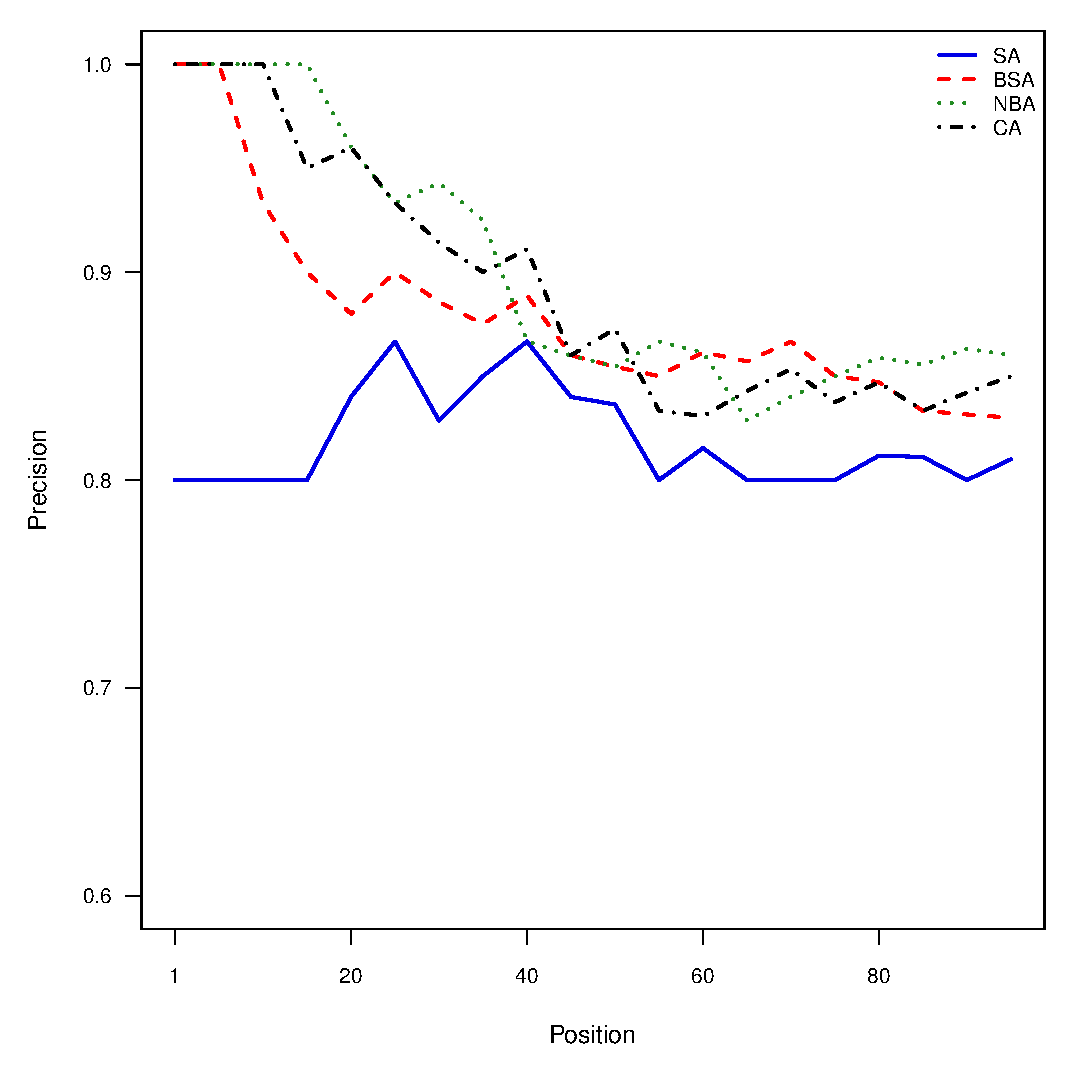
\includegraphics[width=0.45\textwidth]{experiment/e1.ucla.eps}}
\subfigure[MIT]{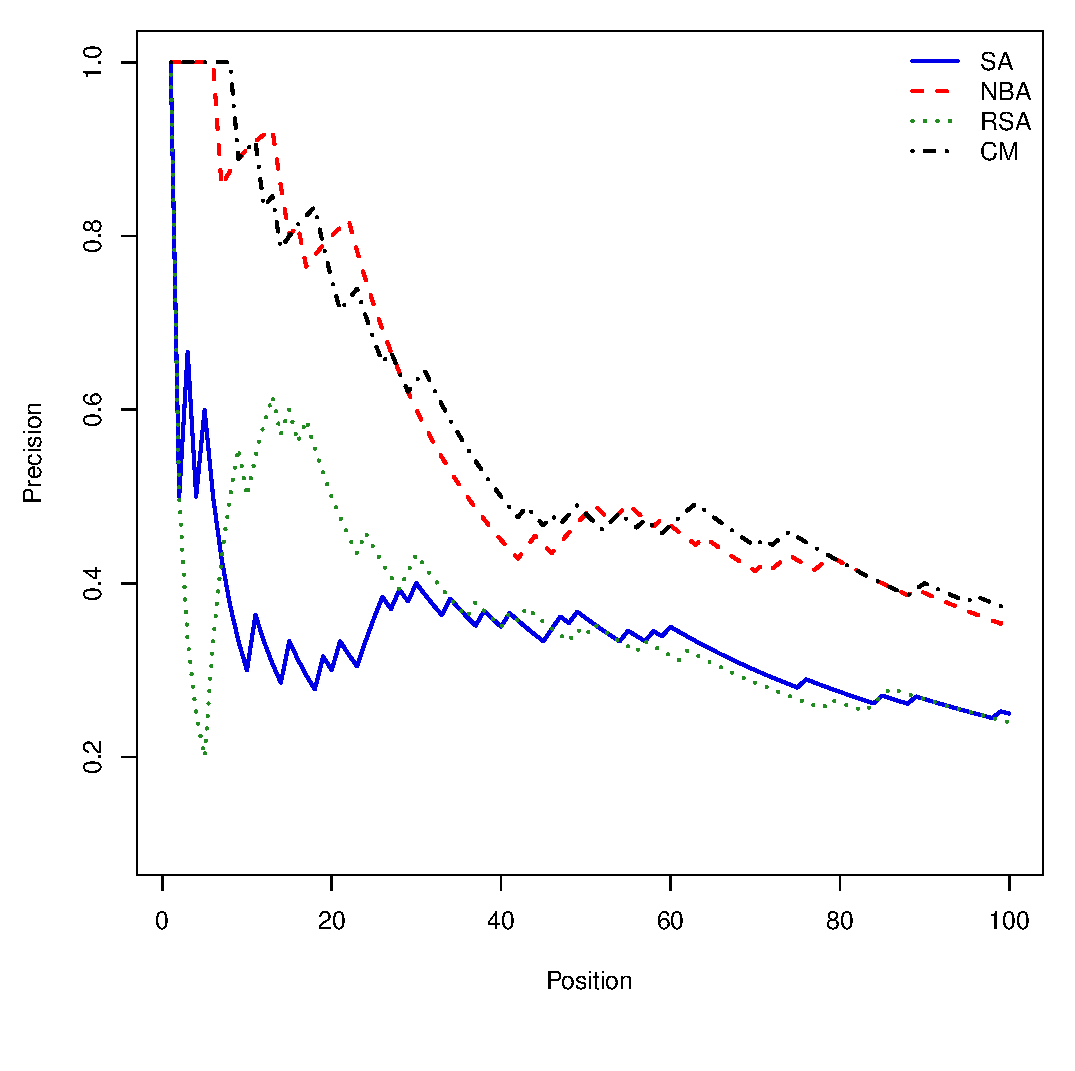
\includegraphics[width=0.45\textwidth]{experiment/e1.mit.eps}}
\\
\subfigure[Stanford]{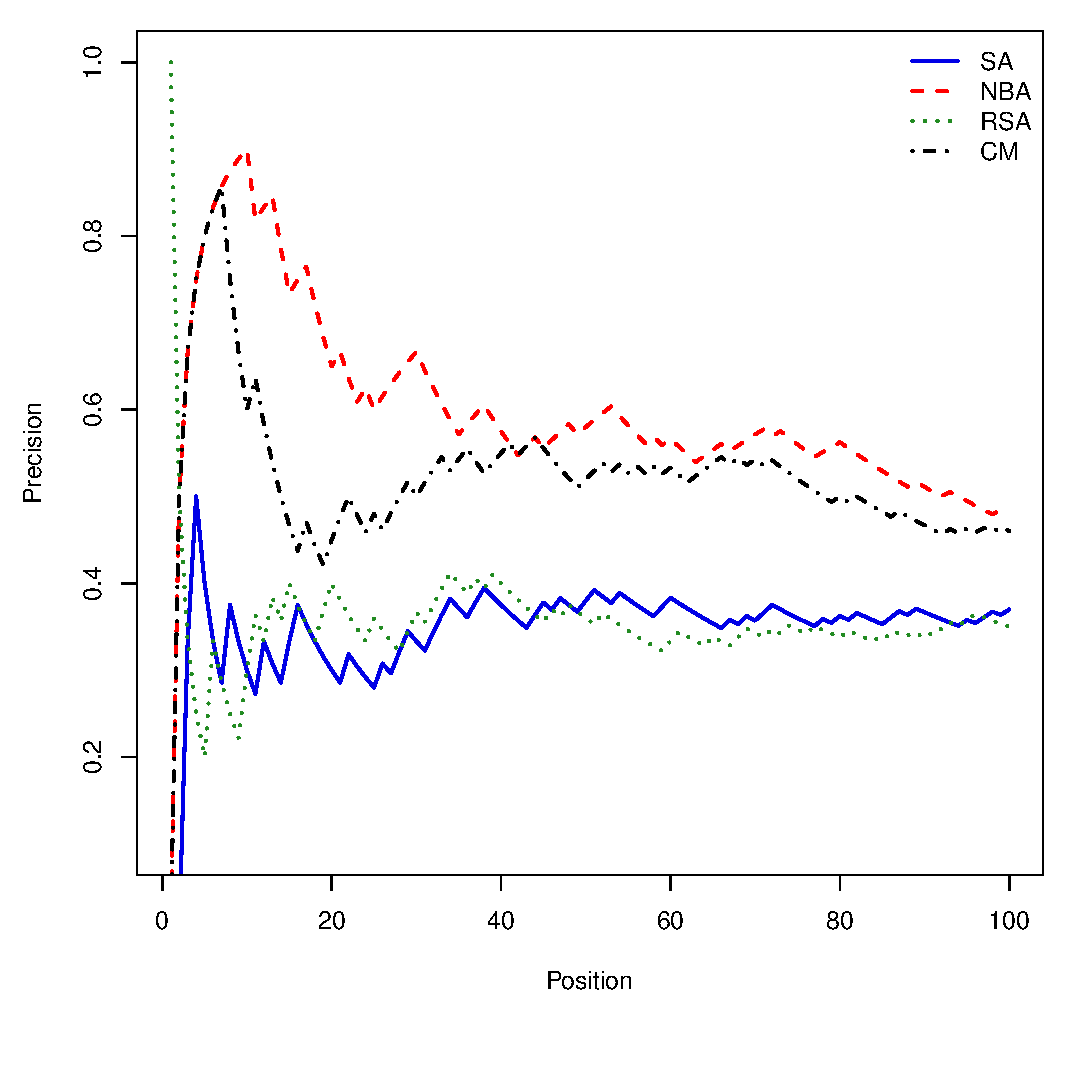
\includegraphics[width=0.45\textwidth]{experiment/e1.stanford.eps}}
\subfigure[USC]{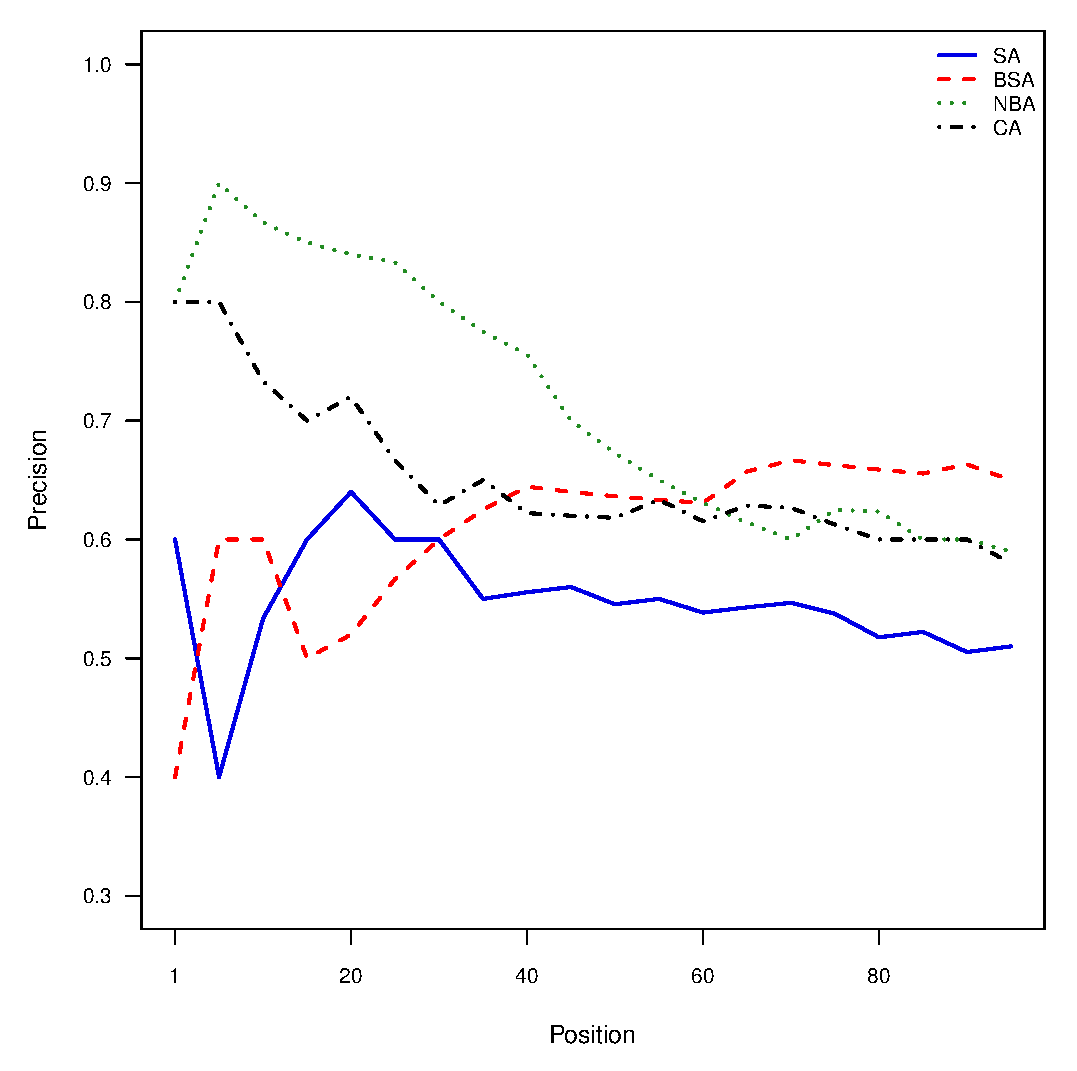
\includegraphics[width=0.45\textwidth]{experiment/e1.usc.eps}}
\caption{Precision\at$k$ for different categories}
\label{fig:e1}
\end{figure*}

From Figure~\ref{fig:e1} we can see that the NBA and CA performs the best at almost every positions. This fact due to the reason that the label data is automated generated by computer. User without category keyword or without large amount of related word will be negative examples in the evaluation. Compare NBA and CA, opposite to our expectation that NBA performs better than CA that is because BSA seriously affected the accuracy of training labels in CA in our computer evaluation system.

The BSA performs better than SA in MIT and USC category, and comparable with SA in Stanford category. But it performs worse than SA in UCLA category, especially in top positions. When we look insight the ranking result, we find that BSA is not as bad as it shows in the figure. For example, the user ranked at the third place in UCLA category is ``LittleBigginKip'', you will find he is a UCLA football team member as soon as you saw his twitter page. However, his profile didn't mention that he is a UCLA student at the time we crawl the data. Moreover, note that much of the improvement in the precision curve in MIT and USC category come in the area after top $10$ positions. This is the area that we most care about, since that users in top position have some features that is easy to discover and users in these middle or tail positions reflect the effectiveness of our algorithm more clearly.

In addition to the keyword based evaluation, Figure~\ref{fig:e2} represents the precision curve in UCLA category on human labeled data. The NBA and CA still performs the best, which shows that users ranked at the top $10$ positions by these algorithms are $100\%$ belong to category UCLA. The BSA performs better than SA since that BSA penalty the users that only interesting to our target category but not actually belong to our target category. For example, the user ``openwestwood'' follows a lot of UCLA stuff which ranked at the $8$th position in SA result but after top 100 positions in BSA result. Actually, after human labeling the experiment result, we find many interesting phenomenons and we will discuss them in our discussion section.
\begin{figure}[htbp]
\centering
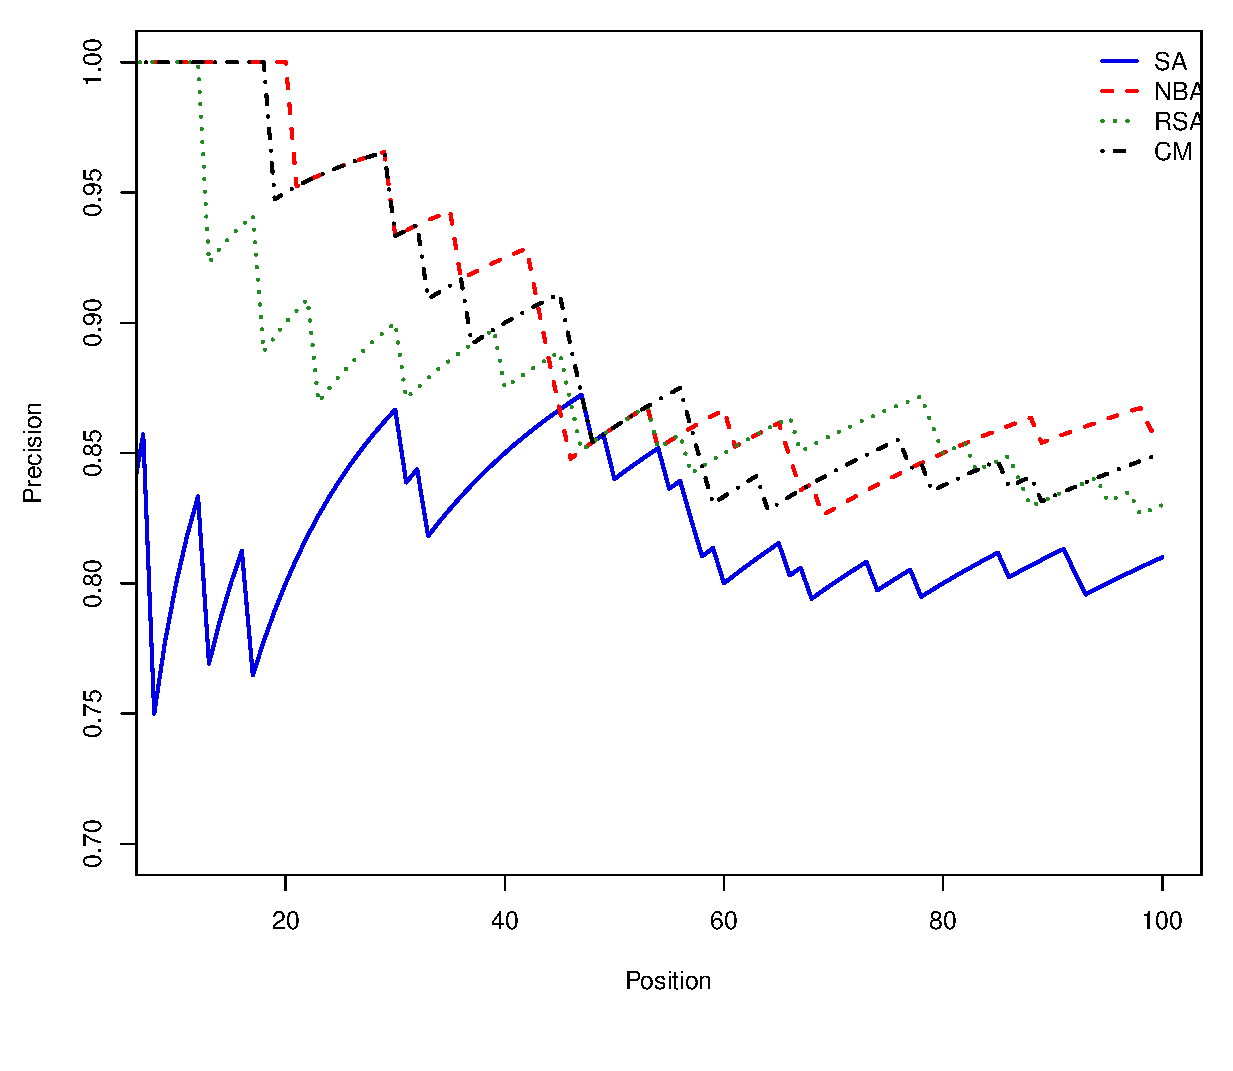
\includegraphics[width=0.45\textwidth]{experiment/e1.ucla.pool.eps}
\caption{Precision\at$k$ for UCLA category on human labeled data}
\label{fig:e2}
\end{figure}

Moreover, we show some important features generated by NBA in Table~\ref{tab:keyword}. The words are ranked according to their occurrence $p(w_i = 1 | c = 1)$, and top 10 words in each category are shown in the table. The top word features for different category are completely different. For example, UCLA students like ``dailybruin'' news, call themselves as ``bruins'' and lived near ``westwood''; USC students like tweets from ``usc annenberge'' and the idol statue in their university is ``Trojan''; MIT students live in ``Cambridge'' and there is famous ``media lab'' in their computer science department; Stanford students are glad to talking about their athletic team using nick name ``cardinal''.

\begin{table*}[htbp]
\centering
\begin{tabular}{|l|l|}
\hline
UCLA & dailybruin, bruin, bruins, westwod, neuheisel, alumna, wooden, undergraduate, midterm, royce \\
\hline
USC & ascj, uscedu, annenberg, uscpsycho, uscannenberg, ausc, beattheirish, trojan, trojans, atrojan \\
\hline
MIT & sloan, medialab, cambridge, joi, kayak, bostonupdate, alums, mechanical, techreview, edu \\
\hline
Stanford & stanfordfball, gostanford, astanford, gsb, cardinal, cantor, tristanwalker, auditorium, alums, freshmen \\
\hline
\end{tabular}
\caption{Top 10 words from user's biography, location and tweets in different universities}\label{tab:keyword}
\end{table*}

\subsection{Ranking with Loss of Information}
In this part of the experiment, the stabilities of different algorithms were tested with loss of information. We randomly selected $1-t\%$ users in $\mathcal{A}$, removed the biography of these users, and moved them to $\mathcal{B}$. The performance of different algorithms under different $t$ is tested, and precision\at$k$ curve is shown in Figure \ref{fig:e3}. SA was not test in this experiment, since its performance is poor in the previous experiment on human labeled data.

\begin{figure}[htbp]
\centering
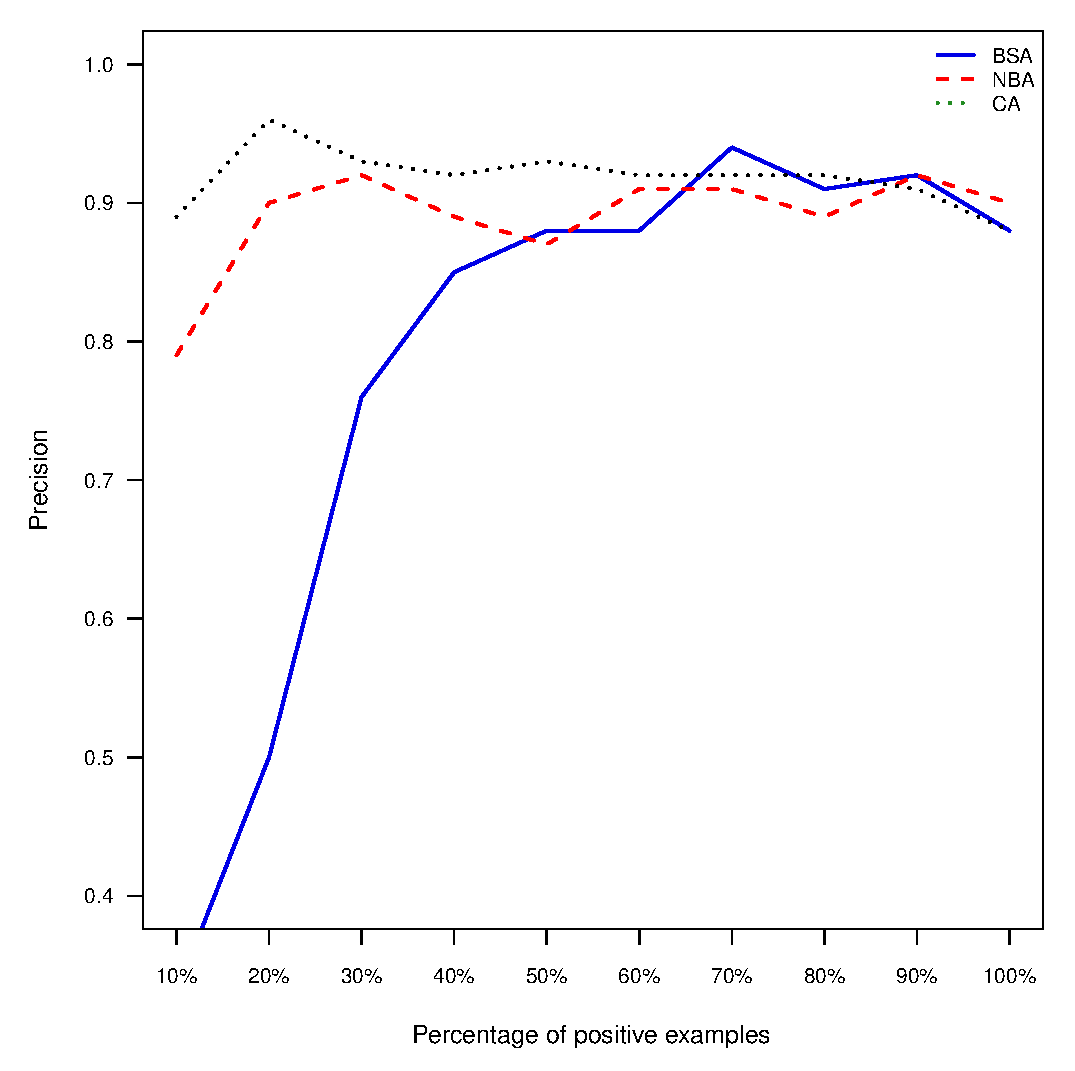
\includegraphics[width=0.45\textwidth]{experiment/e2.ucla.eps}
\caption{Precision\at$k$ for UCLA category with loss of information}
\label{fig:e3}
\end{figure}

The results show that with the loss of information, the performance of BSA falls down dramatically. It also suggests that with few positive training examples, training users in UCLA becomes less connected. The poor graph structure has a bad impact on the performance of BSA.
The NBA still have a very good result with $20\%$ positive training examples. Within those percentage of training users, we could already detect the topic among the tweets published by users belongs to UCLA category. When we look inside the ranking result, the top users returned by BSA and NBA are very accurate. So that the amount of positive training examples does not affect the ranking result of CA very much.

Noticed that sometimes with less positive training examples, our algorithms could achieve better prediction results. That is because when we erase keyword in user's profile, the user is still in our dataset. The total number of users belong to UCLA category in evaluation data increased. So that the precision for top 100 users will be higher.

In our original dataset, the training users are likely to connected with each other since they are in same university. However, for other categories such as father, gamer or phd, users belong to such categories maybe not likely to connected with others in the same category. When we erase the profile keyword in label data, the connection in label data become smaller and the graph structure may like these categories. The performance of our algorithms on UCLA category also demonstrate that our algorithms could be applied to different categories.

\ifx \allfiles \undefined
\end{document}
\fi
\ifx \allfiles \undefined
\documentclass{article}
\usepackage{booktabs}
\usepackage{multirow}
\usepackage{graphicx}
\usepackage{subfigure}

\begin{document}
\title{Discussion}
\maketitle \else \fi

%\subsubsection{Who follows whom on twitter?}
%Table 1 shows the average numbers of followings in different universities with respect to users in different universities. 'Other' represents that the user does not mention any of these four universities in his biography. For example, the third row and second column means 38.17 followings of a UCLA user is in other universities on average. It is shown that the number of followers in the same university is ten times larger than that in different universities. However, this only counts for 5\% among all a user's followers. A possible reason might be that many users do not write their universities in their biographies.

\section{Discussion}\label{sec:discussion}
The manually data labeling process revealed several interesting problems. The top 100 users of UCLA category returned by different algorithms were classified into several categories and described phenomenons as follows.

\subsection{User Classification}
The users are manually classified into $5$ categories, including active users in UCLA with related biography, tweets or photos (ActiveUCLA), inactive users in UCLA (InactiveUCLA), inactive users not belonging to UCLA (Inactive), user intent miss match (Intent), and active user not belonging to UCLA (Negative). The classification result is shown in Figure~\ref{fig:userclass}.

\begin{figure}[htbp]
\centering
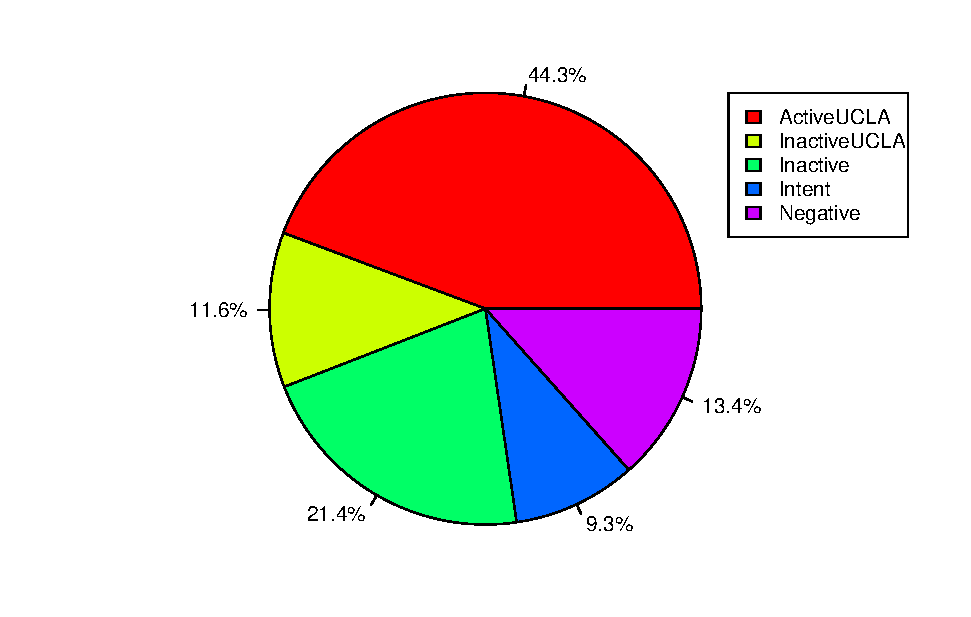
\includegraphics[width=0.5\textwidth]{experiment/uc.eps}
\caption{Manually user classification}
\label{fig:userclass}
\end{figure}

For active users, it is easy to see whether the user has related tweets about UCLA or photos about UCLA. For users without new tweets in recent two months, we call them inactive users and predict whether they are belong to UCLA category according to search result in Google. We type their names with UCLA and see whether there is related search results in top 10 positions.

\subsection{Intent Mismatch}
The intent mismatch, labeled as ``Intent'' in Figure~\ref{fig:userclass}, refers to the situations where the users are somehow interested in UCLA but it is actually not belong to UCLA. The data show that intent mismatch often arises when a user follows a lot of UCLA users or a user talks about something that mentions UCLA.

There are several examples of intent mismatch. First, users may follow UCLA members in order to have more business opportunities, such as ``WeTutorLA'' and ``bombaybite''. The former one follows lot of students from UCLA, USC, UCSD and so on to let them noticed. The latter one follows a lot of organizations of UCLA because it is a restaurant near UCLA. Second, some users keeps follow back a lot of users, such as ``0neNiteStan''. This kind of users have a lot of tweets for advertisement. Third, users like ``USCTrojansNews'', ``openwestwood'' would ranked at higher position in our result. These users' tweets have significant intersection with tweets generated by users from UCLA. For example, ``USCTrojansNews'' often publish tweets that compare UCLA with USC while some users in UCLA category also like to do that. This makes our model make mistakes during the training process.

These kinds of intent mismatch contribute to $9.3\%$ discrepancies in the data. Typically, intent mismatch are very hard to be corrected since it requires human understanding of why this user may related to target category but not belongs to that category.

\subsection{Precision of Active User}

Noticed that there are about $30\%$ users are inactive users. Those users published several tweets after they register and didn't publish any more tweets during recent three months. In real cases, we don't want to see these inactive users since we don't expect that they will provide more information or business opportunity in the future. So that we evaluate our different approaches with inactive user as a negative example and the result is in Figure~\ref{fig:activeprecision}.

\begin{figure}[htbp]
\centering
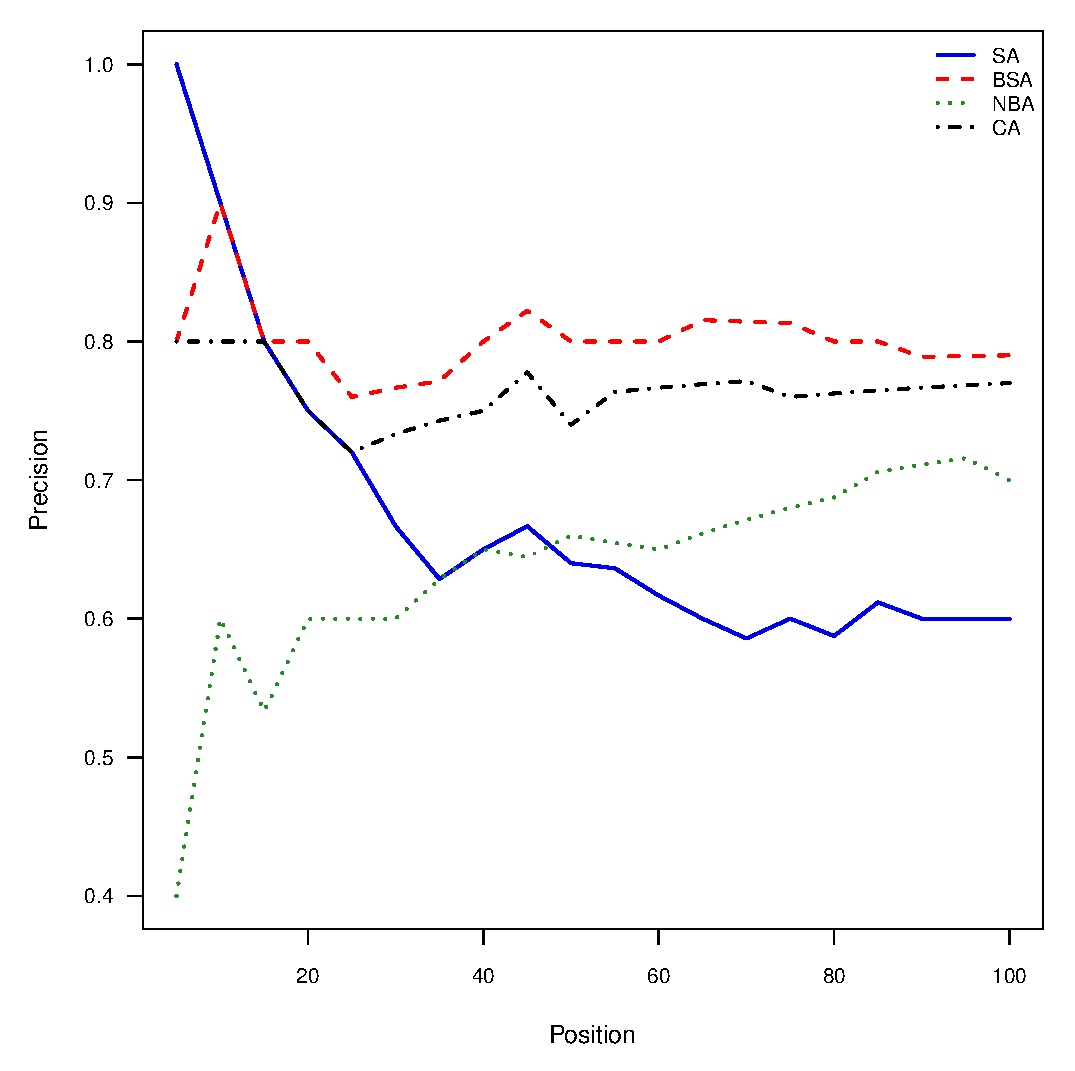
\includegraphics[width=0.45\textwidth]{experiment/ap.eps}
\caption{Precision\at$k$ of active users in UCLA category}
\label{fig:activeprecision}
\end{figure}

Unexpected that SA has the best result and NBA performs the worst in top positions. We look at top users returned by NBA, and found that users such as ``bruinmarketing'' ranked at higher positions by NBA. It seems that ``bruinmarketing'' is in UCLA category, but this user has no tweets among this year. Similarly, some users only mentioned word ``bruin'' in their short bio and ranked higher in NBA turns out to be inactive users.

Moreover, we think that there still exists some disadvantages to treat our task as a classification problem. One disadvantage is that the class is unbalanced. The fraction of positive training samples is too small, which makes the learning particularly difficult. The other disadvantage is the number of features is very large, which is due to the diversity of words user used in their tweets, frequent appearance of typos and hyphen marks.

\ifx \allfiles \undefined
\end{document}
\fi 

\section{Related Work}\label{sec:related-work}
Threshold model

Random Walk Based 

\cite{backstrom2011supervised}

\cite{elo1978rating}

\cite{kwak2010twitter}

\cite{welch2011topical}

\cite{wu2011says}

\cite{yang2011like}

\cite{java2007we}



Granovetter and Schelling were among the first researchers to propose models that capture such a influence propagation process; their approach was based on use of node-specific thresholds \cite{snowball1}, \cite{snowball2}. 
\ifx \allfiles \undefined      
\documentclass{article}
\usepackage{booktabs}
\usepackage{multirow}
\usepackage{graphicx}
\usepackage{subfigure}

\begin{document}
\title{Conclusion}
\maketitle \else \fi

\section{Conclusion}\label{sec:conclusion}
Effectively estimating user profile and accordingly recommending service or suggesting friends are fundamental to all social networks. In this report, we have shown that the user's short bio is highly related with user's friendship information and user's tweets. We presented three simple ranking approaches and a co-training framework that leverage both friendship and tweets evidence to solve the task purposed in our report. The graph approach analysis user profile from his friendship since that similar users are more likely to connected with each other. The Bayes approach extract the semantics of individual message that allow for the generation of user information of a given concept. Given the co-training framework, it is easily for us to combine two different models and obtain a better ranking result with less positive training examples. The experiments results on twitter demonstrate that simple algorithms performs very well for our problem. From the discussion, we learned the pros and cons of different approaches.

The co-training framework that combines graph information and tweets information are not limited to predict user hidden profiles, and can be applied to many other problems that require learning to rank nodes in a graph. There are some interest future research directions: First, the users are equally important in our model based on graph structure. However, we find many inactive users during our labeling process. We may assume users have different weight during the training process. Thus, there may exists the underlying mechanism of how the interactions and information between users related to their personal profile. Second, it is interesting to apply our algorithms in friends recommendation system. Currently, most friend recommendation systems were based on number of users' mutual friends. The co-training approach could leverage users' mutual friends information and other users' behavior such as tweets, profile. I think it is very helpful for building such framework for friends recommendation.

\ifx \allfiles \undefined
\end{document}
\fi


{\bibliography{twitter} \bibliographystyle{plain}}
\end{document}
